\chapter{Development and evaluation of an actuator line model for cross-flow
    turbines}\label{chap:ALM}

To recap, the overarching goal of this work was to find or develop a model for
predicting the performance of arrays of turbines, with a focus on the less
common cross-flow concept. The requirements for this model were:

\begin{enumerate}
    \item Must be able to obtain results for a small array of turbines on a
    typical PC using simulation time on the order of hours per operating
    condition.\label{req:solution-time}
    
    \item Should reasonably match experimental near-wake results for both high
    and low solidity cross-flow turbines with respect to the mean velocity and
    turbulence kinetic energy structure, as well as the relative strengths of
    wake recovery mechanisms. This will ensure our forcing model is a good wake
    generator, and the flow evolution can then be predicted by an accurate flow
    solver and turbulence model.\label{req:wake}
    
    \item Should be able to predict the average performance of a standalone
    turbine to within the accuracy established by blade-resolved 3-D CFD or
    blade element methods.
    
    \item Should match experimental results for the augmented performance of
    turbines in proximity to each other. This is similar to
    requirement~\ref{req:wake}, though from the perspective of turbine's
    response to the flow rather than the flow's response to the turbine.
    
    \item Software should be open-source and not rely on closed-source software,
    if possible.
    
    \item Must be cheaper than physical models for a 3 turbine array. 
\end{enumerate}

With respect to requirement~\ref{req:solution-time}, fast solution times could
be obtained by both momentum and vortex models. However, their poor performance
for high solidity turbines precludes their use \cite{Joo2015}. Furthermore, it
is theoretically impossible for a potential flow vortex method to properly
realize the wake dynamics (requirement~\ref{req:wake})---most importantly the
turbulent transport, which has been shown in both experiment and blade-resolved
CFD to be on the same order of magnitude as the vertical advection. We are
therefore left with Navier--Stokes models.

As we have also seen in Chapter~\ref{chap:CFD}, 2-D blade-resolved CFD could
fulfill solution time requirements, but will never capture vertical advection,
meaning it will also fail to model the performance in an array. Furthermore, 2-D
CFD would not allow for mixed-turbine arrays (AFTs and CFTs). 3-D CFD on the
other hand, would allow for mixed-turbine arrays, could be accurate enough, but
the processing power required would not meet
requirement~\ref{req:solution-time}.

We are then left with actuator-type methods inside Navier--Stokes solvers. As
shown in Chapter~\ref{chap:RVAT-baseline}, the conventional uniform actuator
disk is not a good candidate for a cross-flow turbine wake generator, never mind
the fact that it does not typically compute performance predictions. There are
modified verssions---such as the actuator cylinder---which have been developed
for CFTs \cite{Shamsoddin2014}, though their effectiveness is unknown for 3-D
cases. Finally, the actuator line model (ALM) provides a potential candidate for
meeting all requirements, with the prospect of leveraging continued progress on
improved Navier--Stokes turbulence models. Thus the ALM was chosen for the
present work.

After getting a sense for how two different turbines perform, and how they
affect the flow in which they are placed, the goal is to now develop a way to
predict these effects without resorting to blade-resolved Navier--Stokes CFD.

The blade-resolved CFD work presented in Chapter~\ref{chap:CFD} provided some
targets for what we might expect ideal ALM results to look like inside a RANS
model.

The ultimate goal of the actuator line model is to drive down the computational
costs of simulating turbines by negating the need for complicated meshing, and
the subsequent boundary layer resolution.

The actuator line model, originally developed by Sorensen and Shen
\cite{Sorensen2002}, is based on the classical blade element theory of ???
\todo[inline]{Find citation for creator of blade element theory}
combined with a Navier--Stokes description of the flow field.
The ALM treats turbine blades as lines of blade elements, for which
2-D profile lift and drag coefficients are given. For each blade element,
relative flow velocity and angle of attack are computed by adding the vectors
of relative blade motion and the local fluid velocity. The blade lift and drag
forces are calculated as
\begin{equation}
    F_l = \frac{1}{2} \rho A_\mathrm{elem} C_l |\vec{U}_\mathrm{rel}|^2,
\end{equation}
and
\begin{equation}
    F_d = \frac{1}{2} \rho A_\mathrm{elem} C_d |\vec{U}_\mathrm{rel}|^2,
\end{equation}
where $\rho$ is the fluid density, $A_\mathrm{elem}$ is the blade element
planform area (span $\times$ chord), $\vec{U}_\mathrm{rel}$ is the local
relative velocity, and $C_l$ and $C_d$ are the sectional lift and drag
coefficients, chosen from a table per the local angle of attack. The forces are
then projected onto the rotor coordinate system to calculate torque, overall
drag, etc. Forces from the turbine shaft and blade support struts are computed
in a similar way.

The use of static foil data necessitates corrections for various dynamic effects
induced by the actuator lines rotating within the flow field. Dynamic stall may
be encountered when the blade angle of attack increases past a certain
threshold, and is characterized by an initial increase in lift as a vortex is
shed from the foil's leading edge, after which a drop in lift occurs as the
vortex is advected downstream. Dynamic stall has been shown to be a significant
positive contributor to performance in CFTs \cite{Para2002, Urbina2013},
therefore an accurate model is key. Other dynamic loading considerations stem
from the blade rotation and acceleration---so-called pitching circulation, flow
curvature, and added-mass effects.


\section{Model inputs}

A turbine can be fully described by its geometry, number of elements and their
associated 2-D profiles, and their corresponding coefficient data. Its rotation
can be described by a mean tip speed ratio only, though our earlier experiments
have shown that the cyclic loading of a CFT will cause an oscillation in tip
speed ratio at the blade passage frequency. This oscillation can be described by
an amplitude and phase, similar to how angular velocity was prescribed in
Chapter~\ref{chap:CFD}'s blade-resolved CFD simulations.


\section{Blade element discretization}

In the ALM, a turbine is a collection of actuator lines, which themselves are
collections of actuator line elements (ALEs). The position of each ALE is a
point in space indicating its quarter-chord location. The element is further
defined by its chord direction vector, chord length, span direction vector, span
length, and velocity vector.

An actuator line is created from defined geometry points, between which ALE
parameters are interpolated linearly. This way, an actuator line can be defined
by fewer geometry points than element locations. For example, an AL with
straight planform boundaries---e.g. a straight or tapered wing---only needs two
geometry points to be fully defined. Figure~\ref{fig:AL-geom} shows and example
schematic of a tapered actuator line with three geometry points at the
half-chord locations and six total elements. Note that the middle geometry point
is technically redundant, but is shown for illustrative purposes. For actuator
lines that represent bluff bodies, e.g., shafts, the chord mount offset is set
to 1/4, such that the element location is centered along the line of geometry
points.

\begin{figure}
    \centering
    
    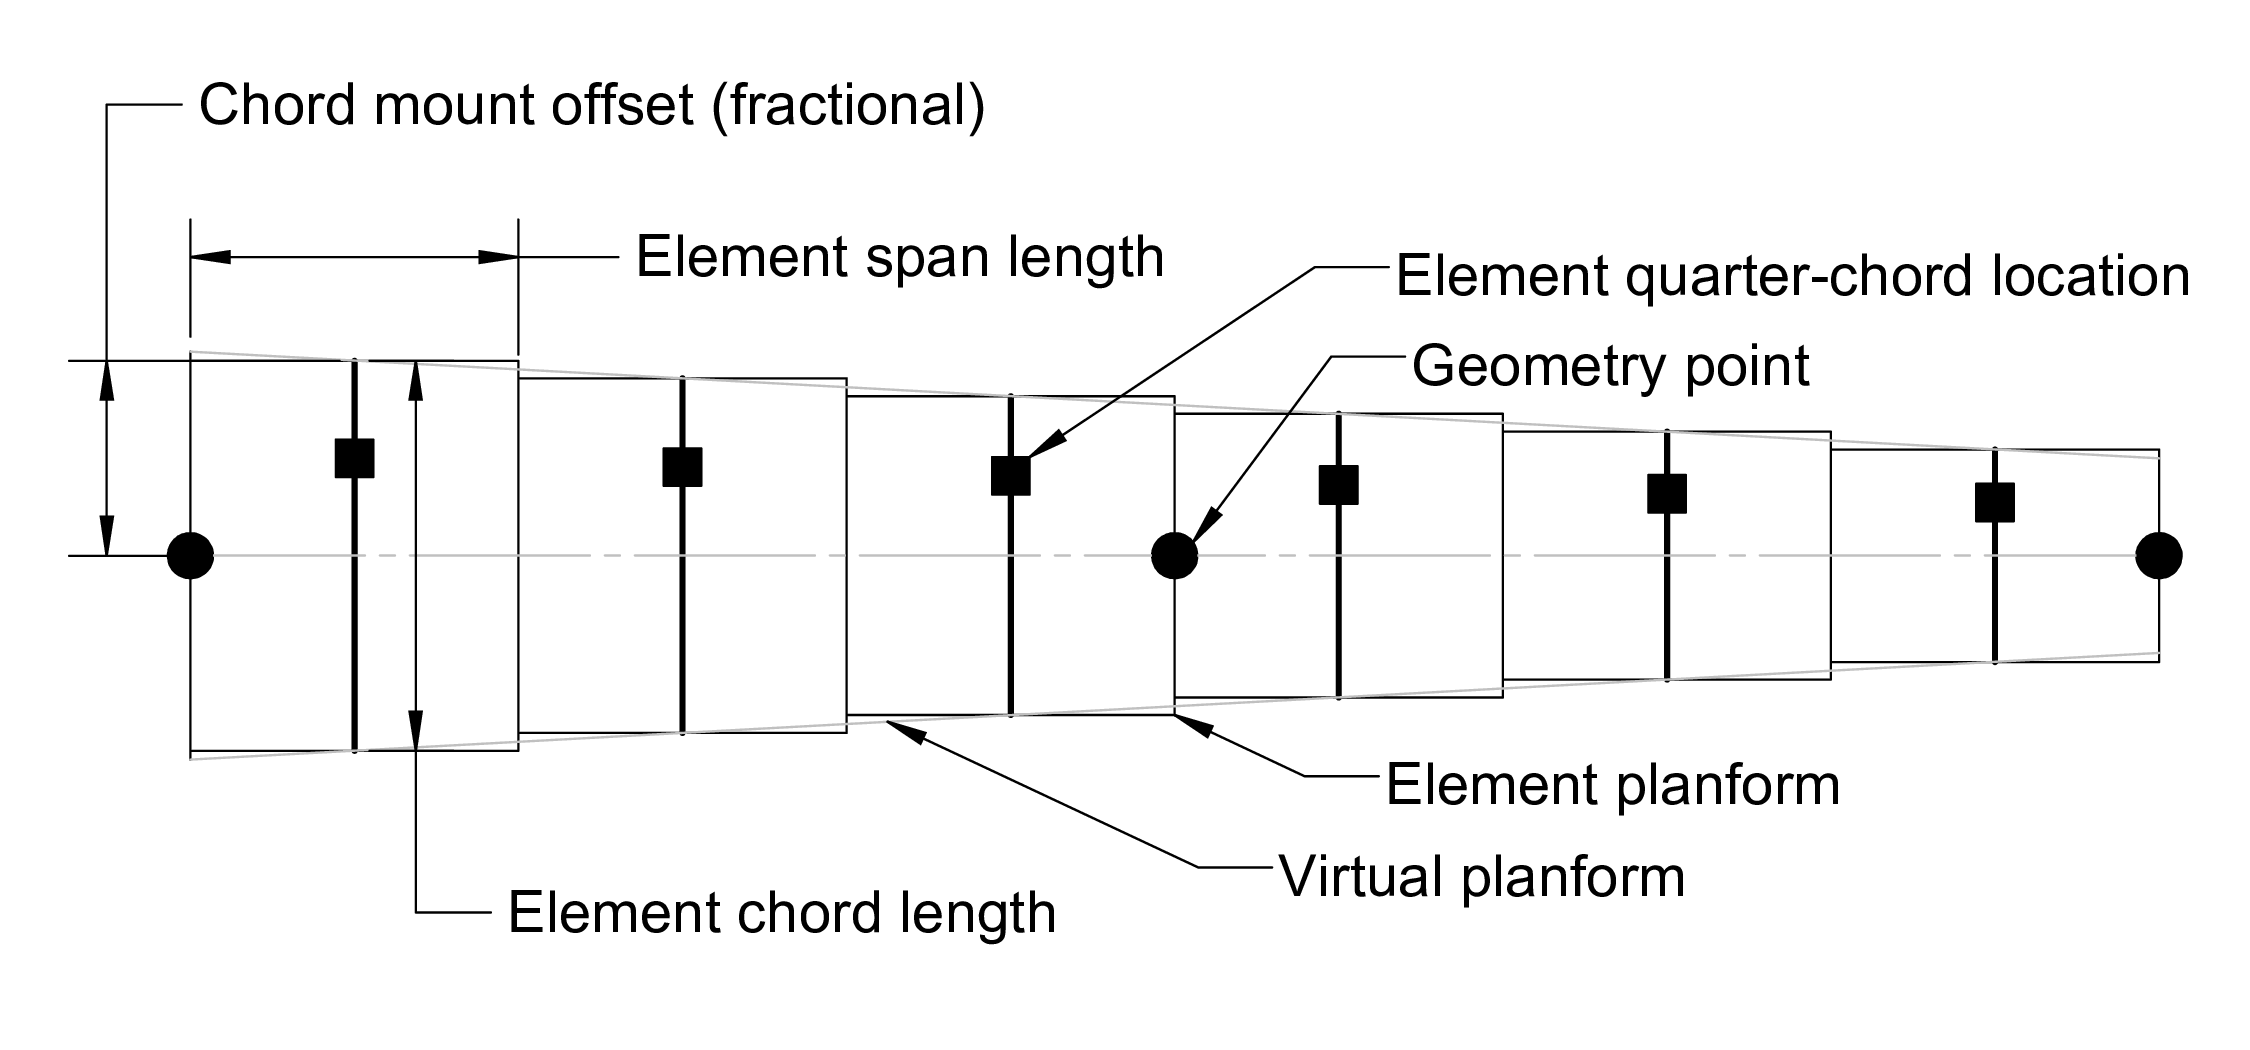
\includegraphics[width=0.9\textwidth]{alm-geometry}
    
    \caption{Actuator line geometry. Filled circles indicate geometry points
        whereas squares indicate actuator line element locations.}
    
    \label{fig:AL-geom}
\end{figure}


\section{Determining inflow velocity}

In momentum methods, the inflow velocity is determined by solving for the axial
and angular induction factors \cite{Manwell2002}. However, using Navier--Stokes
methods, it is somewhat unclear how to calculate the velocity vector used to
compute the angle of attack and relative velocity, though we have access to much
more information about the flow. Sorensen and Shen used an actuator line
element's position to determine the inflow velocity for an axial-flow turbine
\cite{Sorensen2002}. Similarly, Shamsoddin and Porte-Agel use the velocity at a
blade element's location in their actuator line simulation of a vertical-axis
turbine using LES \cite{Shamsoddin2014}. NREL's SOWFA ALM for OpenFOAM also uses
the velocity at the actuator line element location for computing inflow velocity
and local angle of attack with no corrections \cite{Churchfield2013}.

Schito and Zasso developed an effective velocity model (EVM) for computing
actuator forces in Navier--Stokes simulations \cite{Schito2014}. Their EVM
proposes that inflow velocity should be sampled along a line perpendicular to
the mean relative flow direction. They ultimately chose a the line to be 1.5
chord lengths upstream of the actuator point (i.e. quarter-chord location). A
sampling line was chosen to be 5 times the local mesh cell length. Finally, an
angle of attack correction is proposed
\begin{equation}
    \Delta \alpha = \frac{c}{M} (1.2553 - 0.0552 C_d) C_l,
    \label{eq:EVM-dalpha}
\end{equation}
where $c$ is the chord length, $M$ is the mesh size, and $C_l$ and $C_d$ are the
lift and drag coefficients, respectively. Note that the constants in
Equation~\ref{eq:EVM-dalpha} were determined from a calibration with 2-D
blade-resolved CFD for a NACA 0012 foil and are not assumed to be universal.

The EVM, despite showing robustness for its chosen validation case,
unfortunately involves determination of two unknown tuning parameters. To avoid
the additional effort and uncertainty in determining these, the inflow velocity
was sampled at the element quarter-chord location using OpenFOAM's
\texttt{interpolationCellPoint} class, which provides a linear weighted
interpolation using cell values. This algorithm helps keep the sampled velocity
``smooth'' compared with using the cell values themselves, especially when
elements are moving in space as they are in a turbine, since meshes will likely
have a cell size on the same order as the chord length, and will move on the
order of one cell length per time step.


\section{Force projection}

After the force on the ALE from the flow is calculated, it is then projected
back onto the flow field as a source term in the momentum equation. To avoid
instability due to sharp gradients, the source term is tapered from its maximum
value away from the element location by means of a spherical Gaussian function.
The width of this function $\eta$ is controlled by a single parameter
$\epsilon$, which is then multiplied by the actuator line element force and
imparted on a cell with distance $| \vec{r} |$ from the actuator line element
quarter chord location:
\begin{equation}
    \eta = \frac{1}{\epsilon^3 \pi^{3/2}} \exp 
    \left[ - \left( \frac{| \vec{r} |}{\epsilon} \right)^2 \right].
    \label{eq:projection}
\end{equation}

Jha \emph{et al.}~\cite{Jha2014} provides guidelines for choosing a projection
width.

Schito and Zasso \cite{Schito2014} found that a projection $\epsilon$ equal to
the local mesh length was optimal.

Martinez-Tossas and Meneveau \cite{Martinez-Tossas2015b} used a 2-D potential
flow analysis to determine that the optimal projection width for a lifting
surface is 14--25\% of the chord length. The width due to the wake caused by the
foil drag force was recommended to be on the order of the momentum thickness.

Using these guidelines, three length scales were determined: one relative to the
chord length, one to the mesh size, and one to the momentum thickness due to
drag force.

For a bluff body or foil at large angle of attack, drag coefficients are $O(1)$.
The momentum thickness $\theta$ is related to the drag coefficient by
\cite{TennekesAndLumley}
\begin{equation}
    C_d = 2 \theta / l,
    \label{eq:mom-thickness}
\end{equation}
where $l$ is a reference length, e.g., diameter for a cylinder or chord length
for a foil.

Local mesh length was determined as 
\begin{equation}
    \Delta r = 2C_\mathrm{mesh} \sqrt[3]{V_\mathrm{cell}},
\end{equation}
where $V_\mathrm{cell}$ is the volume of the cell containing the actuator line
element, and $C_\mathrm{mesh}$, by default set to 2.0, is a factor to
accommodate cells of non-unity aspect ratio.

Ultimately, an adaptive $\epsilon$ was chosen such that it would be either equal
to $c/4$, or twice the cube root of the volume of the containing cell in the
mesh (roughly equivalent to the $2\Delta r$ recommended by Troldborg
\cite{Troldborg2008}), whichever was larger. This way, fine meshes could benefit
from the increased accuracy of more concentrated momentum sources, and coarse
meshes would be protected from numerical instability.

\todo[inline]{Add final width of Gaussian projection}


\section{Unsteady aerodynamics and dynamic stall}

In the context of a turbine---especially a cross-flow turbine---the actuator
lines will encounter unsteady conditions, both in their angle of attack and
relative velocity. These conditions necessitate the use of unsteady aerodynamic
models to augment the static foil characteristics. Furthermore, the angles of
attack encountered by a CFT blade will often be high enough to encounter dynamic
stall (DS). It is therefore necessary to model both unsteady attached and
detached flow to obtain accurate loading predictions.

\todo[inline]{Discuss Gormont model}

Leishman and Beddoes (LB) developed a semi-empirical model for unsteady
aerodynamics and dynamic stall, which is derived from the phenomenology of the
physics instead rather than pure empiricism \cite{Leishman1989}. Beddoes then
updated the model to the so-called ``3G'' version \cite{Beddoes1993}. Three
variations of this dynamic stall model were tested for cross-flow turbines by
Dyachuk et al. \cite{Dyachuk2014}, with the conclusion that the Sheng et al. low
Mach number modified version \cite{Sheng2008} provided the best results.
Nevertheless, all three models will be implemented and tested in a similar
fashion.

The LB DS models can be summarized conceptually based on the following principles:
\begin{itemize}
    \item Dynamic conditions cause a time lag in effective angle of attack and
    lift force.
    
    \item Dynamic motion can cause an impulsive loading due to added mass
    effects.
    
    \item Separation can be determined by the Kirchoff flow approximation, which
    is also used to parameterize the normal force coefficient table based on the
    trailing edge separation point. This separation point also encounters a time
    lag.
    
    \item The separation initiates a vortex shedding cycle that causes an
    overshoot and subsequent undershoot in lift before returning to an attached
    flow condition.
\end{itemize}


\section{Flow curvature corrections}

The rotating blades of a cross-flow turbine will have varying angle of attack
along their chords for any given azimuthal location due to the circular
path---producing so-called flow curvature effects~\cite{Migliore1980}. This
makes it difficult to define a single angle of attack for use in the static
coefficient lookup tables. Furthermore, this effect is more pronounced for high
solidity ($c/R$) turbines. Two different flow curvature corrections were
considered; one by Goude \cite{Goude2012} and one by Mandal and Burton
\cite{Mandal1994}.

The Goude correction is derived by considering a flat plat moving along a
circular path in potential flow.

\begin{equation}
    \alpha = \delta + \arctan \frac{V_\mathrm{abs} \cos(\theta_b -
        \beta)}{V_\mathrm{abs} \sin(\theta_b - \beta) + \Omega R} - \frac{\Omega
        x_{0r}c}{V_\mathrm{ref}} - \frac{\Omega c}{4 V_\mathrm{ref}},
    \label{eq:Goude-curvature}
\end{equation}
where $\delta$ is the blade pitch angle, $V_\mathrm{abs}$ is the magnitude of
the local inflow velocity at the blade, $\theta_b$ is the blade azimuthal
position, $\beta$ is the direction of the inflow velocity, $\Omega$ is the
turbine's angular velocity, $R$ is the blade element radius, $x_{0r}$ is a
normalized blade attachment point along the chord, $c$ is the blade chord
length, and $V_\mathrm{ref}$ is the reference flow velocity for calculating
angle of attack.

Note that the code uses vector objects and their associated arithmetic in
software (thanks to OpenFOAM's \texttt{vector} class), which means the first two
terms in Equation~\ref{eq:Goude-curvature} are taken care of automatically given
the inflow velocity, chord direction, and element velocity vectors. Therefore,
the last two terms in Equation~\ref{eq:Goude-curvature} was simply added to the
scalar angle of attack. Note that for a cross-flow turbine, this correction
effectively offsets the angle of attack, which therefore increases its magnitude
on the upstream half of the blade path, and decreases its magnitude on the
downstream half, where the angle of attack is negative.

The Mandal--Burton flow curvature correction assumes that since the blade is
encountering a curvilinear flow, it can be treated as having virtual camber.
They introduce a factor to describe the variation of angle of attack from the
leading to trailing edge
\begin{equation}
    \Delta \alpha = \alpha_\mathrm{TE} - \alpha_\mathrm{LE},
    \label{eq:Mandal-Burton-alpha-diff}
\end{equation}
where TE and LE subscripts denote the values of angle of attack at the trailing
and leading edge, respectively. Calculating these values for an actuator line
element can be done by tracking the leading and trailing edge locations and
velocities, then performing the same vector arithmetic used to calculate the
quarter-chord angle of attack.

An incidence correction factor
\begin{equation}
    \alpha_c = \arctan \left( \frac{1 - \cos (\Delta \alpha / 2)}{\sin (\Delta
        \alpha / 2)} \right)
    \label{eq:Mandal-Burton-alpha-corr}
\end{equation}
is introduced and added to the uncorrected angle of attack. Like the Goude
model, $\alpha_c$ is positive on the upstream half of the turbine rotation and
negative on the downstream half. Both implementations are shown in
Listing~\ref{lst:flow-curvature}.

\begin{lstlisting}[float,caption=Flow curvature model implementation.,label=lst:flow-curvature]
    if (flowCurvatureModelName_ == "Goude")
    {
        angleOfAttackRad += omega_*(chordMount_ - 0.25)
                         * chordLength_/mag(relativeVelocity_);
        angleOfAttackRad += omega_*chordLength_/(4*mag(relativeVelocity_));
    }
    else if (flowCurvatureModelName_ == "MandalBurton")
    {
        // Calculate relative velocity at leading and trailing edge
        vector relativeVelocityLE = inflowVelocity_ - velocityLE_;
        vector relativeVelocityTE = inflowVelocity_ - velocityTE_;
    
        // Calculate vector normal to chord--span plane
        vector planformNormal = -chordDirection_ ^ spanDirection_;
        planformNormal /= mag(planformNormal);
        
        // Calculate angle of attack at leading and trailing edge
        scalar alphaLE = asin((planformNormal & relativeVelocityLE)
                       / (mag(planformNormal)*mag(relativeVelocityLE)));
        scalar alphaTE = asin((planformNormal & relativeVelocityTE)
                       / (mag(planformNormal)*mag(relativeVelocityTE)));
        
        scalar beta = alphaTE - alphaLE;
        
        angleOfAttackRad += atan2((1.0 - cos(beta/2.0)), sin(beta/2.0));
    }
\end{lstlisting}


\section{End effects}

Foils of finite span will not have uniform load distributions.

Glauert used Prandtl's lifting line theory to develop a tip loss correction
factor for an axial-flow rotor. This has been further developed by Shen et al.
\cite{Shen2005a}. However, we seek a correction model that does not depend on
the rotor context, such that the model could be used for axial- and cross-flow
turbines, along with standalone actuator lines, e.g. wings.

From Prandtl's lifting line theory, the geometric angle of attack $\alpha$ of a
foil with an arbitrary circulation distribution can be expressed as a function
of nondimensional span $\theta$ as \cite{Anderson2001}
\begin{equation}
    \alpha (\theta) = \frac{2S}{\pi c (\theta)}
    \sum_1^N A_n \sin \theta
    + \sum_1^N n A_n \frac{\sin n \theta}{\sin \theta}
    + \alpha_{L = 0}(\theta),
    \label{eq:lifting-line}
\end{equation}
where $S$ is the span length, $c(\theta)$ is the chord length, and $N$ is the
number of locations or elements sampled along the foil. This relationship can be
rearranged into a matrix equation to solve for the unknown Fourier coefficients
$A_n$,
\begin{equation}
    [\alpha_m ] - \alpha_{L=0} = [D_{mn}][A_n],
\end{equation}
where
\begin{equation}
    D_{mn} = \sum_1^N \left[ \frac{2b}{\pi c_m} \sin n \theta_m + n \frac{\sin n
        \theta_m}{\sin \theta_m} \right].
\end{equation}

With the Fourier coefficients, the circulation distribution can be calculated as
\begin{equation}
    \Gamma (\theta) = 2SU_\infty \sum_1^N A_n \sin n \theta,
\end{equation}
which, via the Kutta--Joukowski theorem, provides the lift coefficient
distribution
\begin{equation}
    C_l(\theta) = \frac{-\Gamma (\theta)}{\frac{1}{2} c U_\infty}.
\end{equation}

We can therefore compute a correction function 
\begin{equation}
    F = C_l(\theta)/C_l(\theta)_{\max},
\end{equation}
which will be in the range $[0, 1]$, similar to the Glauert corrections, but
does not contain rotor parameters. The correction function for various methods
is compared in Figure~\ref{fig:end-effects}.

\begin{figure}
    \centering
    
    \caption{End effect correction function values for the Glauert, Shen et al.,
        and lifting line methods.}
    
    \label{fig:end-effects}
\end{figure}



\section{Reynolds number corrections}

As seen in Chapter~\ref{chap:Re-dep}, Reynolds number can have significant
effects on turbine performance below a threshold value. To maintain accuracy
using a single static foil data table in a flow of varying inflow velocity
magnitude, Reynolds number corrections should be applied. Yamauchi and Johnson
\cite{Yamauchi1983} proposed a simple correction derived from turbulent flat
plate boundary layer results, where the drag coefficient is corrected as
\begin{equation}
    C_d = C_{d_{\mathrm{table}}}/ K,
    \label{eq:cd-correction}
\end{equation}
where $K = f(Re_\mathrm{table})/f(Re)$. There are several choices for the
scaling function $f(Re)$:
\begin{equation}
    f(Re) = Re^{-0.5},
\end{equation}
\begin{equation}
    f(Re) = Re^{-0.2},
\end{equation}
\begin{equation}
    f(Re) = \frac{0.455}{\ln Re}2.58 - \frac{A}{Re},
\end{equation}
\begin{equation}
    f(Re) = (3.46 \ln Re - 5.6)^{-2},
\end{equation}
or
\begin{equation}
    f(Re) = (\ln Re - 0.407)^{-2.64}.
\end{equation}

Yamauchi and Johnson propose a correction for the lift coefficient that will
keep the lift slope constant, i.e.
\begin{equation}
    C_l = K C_{l_\mathrm{table}} (\alpha/K),
\end{equation}
where
\begin{equation}
    K = \alpha_{\max} / \alpha_{\max_\mathrm{table}} = C_{l_{\max}} /
    C_{l_{\max_\mathrm{table}}}.
\end{equation}
The scaling constant is chosen as
\begin{equation}
    K = \left( Re/Re_\mathrm{table} \right)^n,
\end{equation}
where $n$ is a small positive number between approximately 0.125 and 0.2.

Figure~\ref{fig:Re-corrections} shows the results of the chosen Reynolds number
correction compared with foil data taken at multiple $Re$.

\begin{figure}
\caption{Reynolds number corrections compared with foil data acquired at
multiple Reynolds numbers.}
\label{fig:Re-corrections}
\end{figure}

Note that these Reynolds number corrections are applied before the dynamic stall
model, such that the changes in e.g. the Kirchoff flow equation fit parameters
$S_1$ and $S_2$ will be changed automatically as well.


\section{Effects on turbulence modeling}

Conventional blade element simulations use either momentum or vortex methods to
solve for the incident flow field, and these methods do not model the effects of
turbulence. With the actuator line model, there is the opportunity to improve
the physical realism by not only adding a source to the momentum equations, but
also to the turbulence model equations.

James et al. implemented an actuator disk model in a RANS model with a
$k$--$\epsilon$ closure, which ``injected'' $k$ and $\epsilon$ from the actuator
disks to more realistically simulate the turbine's turbulent wake and enhance
momentum transport \cite{James2010}. However, to the author's knowledge
injecting turbulence quantities has never been done in an actuator line model.

In this case, we seek to inject turbulence dependent on blade loading, both
for the $k$--$\epsilon$ RANS model and the
\todo[inline]{Pick LES model to work with.}

Turbulence sources were calibrated by simulating a 2-D symmetrical NACA airfoil
using the $k$--$\omega$ SST turbulence model, given its strength at predicting
stall. We seek a turbulence injection rate as a function of drag coefficient, as
this should be a good indicator of flow separation, where production of
turbulence will be greatly increased.

An automated OpenFOAM case was developed to perform the turbulence injection
calibration. This case automatically created a \texttt{blockMeshDict} for a
given NACA foil at specified angle of attack, ran the simulation until
convergence, then sampled and logged the lift, drag, moment coefficients, along
with the maximum values and locations of $k$, $\omega$, and $\epsilon$ 1.25
chords downstream of the leading edge.

\begin{figure}[ht]
    \centering
    
    \caption{2-D NACA 0021 foil mesh at 20 degrees angle of attack.}
    
    \label{fig:NACA-foil-mesh}
\end{figure}


\begin{figure}[ht]
    \centering
    
    \caption{Turbulence kinetic energy computed around the 2-D NACA 0021 foil at
        20 degrees angle of attack.}
    
    \label{fig:NACA-foil-k}
\end{figure}


\begin{figure}[ht]
    \centering
    
    \caption{Simulated drag coefficient and turbulence quantities plotted versus
        angle of attack for a 2-D NACA 0021.}
    
    \label{fig:NACA-foil-turbulence}
\end{figure}


\section{Software implementation}

The ALM was written as an extension library for the OpenFOAM free and
open-source CFD library. OpenFOAM is in general a package for solving partial
differential equations using the finite volume method. However, it contains many
pre-built applications for meshing, pre-processing, solving, and post-processing
CFD simulations. The library contains implementations of models for compressible
and incompressible flow, turbulence via RANS, LES, and detached eddy simulation
(DES), multiphase flows, dynamic mesh handling, and more, making it a very
powerful general purpose simulation framework, capable of easily scaling to
massively parallel high performance computing clusters. OpenFOAM is also widely
used throughout industry and academia. As shown in Figure~\ref{fig:cfd-online},
OpenFOAM has the second highest number of discussion threads, but a much higher
post-per-thread count compared to other popular discussion forums on
CFD-online.com. This greater community involvement makes OpenFOAM a perfect
library in which to integrate this model, with respect to potential impact,
adoption, and collaboration.

\begin{figure}[ht]
    \centering
    
    \includegraphics[width=0.95\textwidth]{figures/CFD-pop_cfd-online}
    
    \caption{Total number of threads (left) and posts-per-thread for the four
        most popular forums on CFD-online.com as of September 27, 2015.}
    
    \label{fig:cfd-online}
\end{figure}

The code will be written in OpenFOAM's style, similar to NREL's SOWFA, but will
use OpenFOAM's \texttt{fvOptions} framework for adding source terms to equations
at runtime---see Listing~\ref{lst:fvOptions} for an example implementation with
the momentum equation. This strategy will allow the CFT-ALM to be added to many
of the solvers included in OpenFOAM, meaning it can be readily used with RANS or
LES, multiphase models (e.g. for simulating the free surface in MHK
installations), and even with heat transfer. Furthermore, unlike SOWFA, custom
solvers will not need to be developed to include the CFT-ALM. It is also likely
that the extension library developed here will be expanded to include axial flow
turbine models similar to SOWFA.

Since all applications are run from a command line and all input data is text
based, automation and integration with other tools is relatively
straightforward. Future enhancements could include cooperation with software for
generating static foil data, e.g., XFOIL or other OpenFOAM solvers, turbine
controller models, structural analysis codes, and optimization tools, e.g.,
SNL's DAKOTA, for both individual turbines and array layouts.

\begin{lstlisting}[float,caption=Adding source terms to the momentum equation in OpenFOAM.,label=lst:fvOptions]
tmp<fvVectorMatrix> UEqn
(
    fvm::ddt(U)
    + fvm::div(phi, U)
    + turbulence->divDevReff(U)
    ==
    fvOptions(U)
);
\end{lstlisting}


\subsection{Object orientation}

C++ permits the object oriented programming paradigm, which helps modularize
code for increased readability and reuse. In \textit{turbinesFoam}, a turbine is
a software object that is composed of actuator line objects, which themselves
are composed of actuator line element objects. Structuring the code this way
allows testing of the functionality of individual components. For example, an
actuator line can be tested outside the turbine context to ensure is produces
the correct forcing, without adding the complexity of rotation, other actuator
lines, etc. that would be present in a turbine rotor. In contrast, the actuator
line model in \textit{SOWFA} uses a single software object to represent an
entire array of turbines. This architecture necessitates iterating through many
nested lists down to the element level, which can be confusing to read.


\subsection{Parallelization}

OpenFOAM's custom container classes and loop macros were used wherever possible
to aid in parallelization.


\section{Results}

In this section results are presented for cases used to verify various
sub-models, and finally test the ALM against the experimental targets.

\todo[inline]{Discuss verification}


\subsection{High solidity cross-flow turbine}

The UNH-RVAT was chosen as a high solidity CFT case for model validation, thanks
to our earlier experimental and numerical investigations.

\todo[inline]{Describe end effects model settings for RVAT.}


\subsubsection{Performance prediction}

Power and drag coefficient curves are plotted for the UNH-RVAT in
Figure~\ref{fig:RVAT-ALM-perf-curves}. The ALM does a good job predicting the
drag coefficient, along with the power coefficient at low tip speed ratios, but
overpredicts $C_P$ at high $\lambda$. This may be caused by the physical model
turbine having exposed bolt heads and other imperfections located far enough
from the axis to have a large parasitic effect at high rotation rates. In
Chapter~\ref{chap:RM2} we showed how these losses can be significant even with
carefully smoothed struts and strut-blade connections.

\begin{figure}
    \caption{Power and drag coefficient curves computed for the UNH-RVAT using
        the Leishman--Beddoes model modified by Sheng et al.}
    
    \label{fig:RVAT-ALM-perf-curves}
\end{figure}


\subsubsection{Wake characteristics}

Figure~\ref{fig:RVAT-ALM-meancontquiv-DS} shows mean velocity field for the
UNH-RVAT computed by the ALM with and without the Leishman--Beddoes dynamic
stall model modified by Sheng et al. (the LB-SGC model). We see how the
directions of the effects of tip vortices are opposite.

\begin{figure}
    \caption{Mean velocity field at $x/D=1$ with no dynamic stall model and the
        LB-SGC model.}
    
    \label{fig:RVAT-ALM-meancontquiv-DS}
\end{figure}

The sensitivity of the wake's mean flow structure was also tested with respect
to flow curvature correction for blade loading, the results for which are
plotted in Figure~\ref{fig:RVAT-ALM-flow-curvature}. Like the dynamic stall
model, the chosen curvature correction can have a significant effect on the
location at which tip vortices are strongest, which in turn affects the
qualitative structure of the mean flow in the near-wake.

\begin{figure}
    \caption{Mean velocity field at $x/D=1$ with the LB-SGC model, with and
        without the Goude flow curvature correction.}
    
    \label{fig:RVAT-ALM-flow-curvature}
\end{figure}

Turbulence kinetic energy contours (including resolved and modeled energy) are
shown in Figure~\ref{fig:RVAT-ALM-kcont}. We see that without the turbulence
injection model active, the vertical band of $k$ on the $-y$ side of the
turbine---caused by dynamic stall---is missing.

\begin{figure}
    \caption{Turbulence kinetic energy contours at $x/D=1$ with an without
        turbulence injection activated.}
    
    \label{fig:RVAT-ALM-kcont}
\end{figure}

Weighted averages for the momentum recovery terms are tallied in
Figure~\ref{fig:RVAT-ALM-recovery}.

\begin{figure}
    \caption{Weighted average momentum recovery terms for the UNH-RVAT in the
        ALM with a $k$--$\epsilon$ closure.}
    
    \label{fig:RVAT-ALM-recovery}
\end{figure}


\subsection{Low solidity cross-flow turbine}

The RM2 low solidity cross-flow turbine is another good validation case given
its differences from the UNH-RVAT. 

\todo[inline]{Describe end effects model settings for RM2.}

Figure~\ref{fig:RM2-ALM-perf-curves} presents
the performance curves computed by the ALM, and those from the tow tank
experiments. As with the high solidity RVAT, the drop in $C_P$ comes at higher
$\lambda$.

\begin{figure}
    \caption{Power and drag coefficient curves computed for the RM2 using the
        LB-SGC model.}
    
    \label{fig:RM2-ALM-perf-curves}
\end{figure}

Since the RM2 dataset contained measurements with no blades and both high and
low drag struts. The RM2 was also simulated in these conditions to assess how
well the actuator line model can predict the losses due to strut drag, which may
be a partial explanation for why the power coefficient does not drop off at high
$\lambda$ as quickly as in the experiments. Performance curves without blades
are shown in Figure~\ref{fig:RM2-ALM-strut-perf}.

\begin{figure}
    \caption{Turbine performance curve with no blades, with NACA 0021 (a) and
        cylindrical (b) struts.}
    
    \label{fig:RM2-ALM-strut-perf}
\end{figure}

Figure~\ref{fig:RM2-ALM-flow-curvature} shows the mean velocity field computed
for the low solidity RM2 cross-flow turbine with the two different flow
curvature corrections. We see that with the Goude correction, the location of
the maximum streamwise velocity deficit is shifted rightward, whereas the
experimental results showed that the profile was more-or-less symmetrical. This
essentially tells us that the Goude model is more effective for the high
solidity RVAT, though the low solidity RM2 may not need flow curvature
corrections to obtain accurate results.

\begin{figure}
    \caption{Mean velocity field at $x/D=0.93$ for the RM2, with the Goude and
        Mandal--Burton flow curvature corrections.}
    
    \label{fig:RM2-ALM-flow-curvature}
\end{figure}


\subsection{UNH-RVAT LES}

\todo[inline]{Discuss mesh resolution determination.}

Thanks to the ALM's general implementation as a source term, we are not tied to
any specific turbulence model. This means that as turbulence modeling and
computational power advance, the ALM can continue to be used. As a look towards
the future prospect of simulating large CFT arrays in great detail, a single CFT
was placed in a large eddy simulation (LES). Turbine geometry was identical to
the UNH-RVAT case, but the domain was extended to look at wake evolution father
downstream.

To perform the LES, the spatio-temporal grid was refined in order to resolve
more of the turbulent energy spectrum. Pope \cite{Pope2000} recommends 10--20
Kolmogorov length/time scales, which can be estimated as
\begin{equation}
    \eta = ( \nu^3 / \epsilon )^{1/4},
    \label{eq:Kolmogorov-length}
\end{equation}
and
\begin{equation}
    \tau = ( \nu / \epsilon )^{1/2},
    \label{eq:Kolmogorov-time}
\end{equation}
respectively. The dissipation $\epsilon$ was estimated as $\sigma_u^3/l$, where
$\sigma_u$ is the velocity standard deviation, estimated from a low inflow
turbulence intensity of XXX \todo[inline]{Estimate inflow turbulence}, and $l$,
the turbulent length scale, was estimated to be 10 cm.

\begin{figure}
    \caption{Snapshot of vorticity contours for the UNH-RVAT LES case.}
    
    \label{RVAT-LES}
\end{figure}

\todo[inline]{Add meancontquiv for RVAT LES case?}

\todo[inline]{Add recovery terms for RVAT LES case?}


\section{Computational cost}

\todo[inline]{Move this section to conclusions or top-level results section like
    CFD chapter.}

Compared to blade-resolved RANS, the ALM can solve a standalone turbine case on
the order of CPU minutes per second of simulated time versus 1,000 CPU hours per
second---a savings of 4 orders of magnitude. However, the results for the ALM
are not quite as detailed. For example, the $-y$ tip vortex (where dynamic stall
is occurring) is not captured by the ALM.


\section{Conclusions}

In this chapter the actuator line model has been developed and tested against
the cross-flow turbine validation datasets acquired in previous chapters.

With respect to the model's goals...

Despite a small loss in accuracy, the ALM can do a reasonable job predicting the
performance and wake of a cross-flow turbine. It is therefore expected that this
tool will provide a much improved means of designing array layouts compared with
simple actuator disks, point sources, or superposition techniques---and all with
acceptable computational cost, i.e., not requiring HPC resources.

%%% Below from proposal introduction

If the proposed body force model is inadequate for postdicting our experimental
performance data, one possible strategy for improving accuracy is to generate
foil coefficient databases with more dimensions, e.g., blade pitch rate or local
turbulence levels. It may also be possible to modify the dynamic loading models
based on insight from the body-fitted grid simulations.
